\subsubsection{Valor del torque necesario}

El torque nominal en un motor de corriente continua representa el par o
fuerza de rotación que el motor puede entregar de manera continua y segura
sin sobrecalentarse o dañarse. Es el valor de torque que el motor está diseñado
para proporcionar bajo condiciones normales de operación, es decir, cuando
funciona a su voltaje y corriente nominales.
Calculamos el torque mínimo necesario que debe soportar el motor:
\[
A_{\text{cortina}} = \SI{1,2}{\meter} \cdot \SI{1,4}{\meter} = \SI{1,68}{\meter\squared}
\]

Siendo la densidad superficial del lino:

\[
\delta_{\text{Lino}} = \SI{0,2}{\kilogram\per\square\meter}
\]

Entonces:

\[
P_{\text{Lino}} = \delta_{\text{Lino}} \cdot A_{\text{cortina}} = \SI{0,2}{\kilogram\per\square\meter} \cdot \SI{1,68}{\square\meter} = \SI{0,336}{\kilogram}
\]

Por lo tanto, el peso total es:

\[
P_{\text{Total}} = P_{\text{cortina}} + P_{\text{palo}} = \SI{0,336}{\kilogram} + \SI{1}{\kilogram} = \SI{1,336}{\kilogram}
\]

La fuerza total:

\[
F_{\text{total}} = P_{\text{Total}} \cdot g = \SI{1,336}{\kilogram} \cdot \SI{9,8}{\meter\per\second\squared} = \SI{13,09}{\newton}
\]

Finalmente, el torque necesario:

\[
\tau = F \cdot r_{\text{eje}} = \SI{13,09}{\newton} \cdot \SI{0,015}{\meter} = \SI{0,1964}{\newton\meter} = \SI{196,4}{\milli\newton\meter}
\]

Una de las razones por las cuales se agrega la caja reductora es adaptar el torque del motor al necesario para la cortina, observando la hoja de datos del motor vemos que el valor de torque nominal del mismo es de $\SI{32}{\milli\newton\meter}$ a partir de este valor se determina la relación de transmisión mínima necesaria $N$:

\[
N = \frac{\tau_{necesario}}{\tau_{nominal}} = \frac{\SI{196,4}{\milli\newton\meter}}{\SI{32}{\milli\newton\meter}} = 6,13
\]

Por lo tanto es necesario una caja reductora con \textbf{una relación de transmisión de $N>7$ para cumplir con el torque} y de esta forma que el motor opere de manera segura y eficiente.

\subsubsection{Adaptación del momento de inercia}

Además del requerimiento de torque estático, es fundamental analizar la dinámica del sistema. Para que el sistema sea estable y el motor pueda acelerar la carga sin saturarse, se busca un adecuado acoplamiento de impedancias mecánicas.

Primero, modelamos la inercia de la carga ($J_{\text{carga}}$) considerando la cortina como un cilindro macizo y sumando la inercia del eje. Utilizando la masa total ($P_{\text{Total}}$) y el radio ($r_{\text{eje}}$):

\[
J_{\text{carga}} = \frac{1}{2} \cdot P_{\text{Total}} \cdot r_{\text{eje}}^2
\]

\[
J_{\text{carga}} = \frac{1}{2} \cdot \SI{1,336}{\kilogram} \cdot (\SI{0,015}{\meter})^2 = \SI{1,503e-4}{\kilogram\meter\squared}
\]

Observando la hoja de datos del motor, la inercia del rotor del motor es $\SI{1,0e-6}{\kilogram\meter\squared}$


Si conectáramos el motor directamente ($N=1$), la relación de inercias sería de $150:1$, lo cual haría el sistema incontrolable. Para garantizar una respuesta dinámica óptima, se aplica el criterio de \textit{Inertia Matching}, buscando que la inercia reflejada de la carga sea menor o comparable a la inercia del motor. Planteamos la condición ideal donde la inercia reflejada es igual a la inercia del motor:

\[
\frac{J_{\text{carga}}}{N^2} \leq J_{\text{motor}}
\]

Despejando $N$ para encontrar la relación de transmisión mínima necesaria por criterios dinámicos:

\[
N \geq \sqrt{\frac{J_{\text{carga}}}{J_{\text{motor}}}} = \sqrt{\frac{\SI{1,503e-4}{\kilogram\meter\squared}}{\SI{1,0e-6}{\kilogram\meter\squared}}}
\]

\[
N \geq \sqrt{150,3} \approx 12,26
\]

El criterio de inercia ($N>13$) es más restrictivo que en el caso del torque estático ($N>7$). Por lo tanto, para cumplir ambas condiciones con holgura y asegurar robustez, se selecciona una caja reductora con una relación de transmisión de \textbf{40:1} ($N=40$).

Finalmente, la inercia total equivalente vista por el eje del motor será:

\[
J_{\text{eq}} = J_{\text{motor}} + \frac{J_{\text{carga}}}{N^2} = \SI{1,0e-6}{} + \frac{\SI{1,503e-4}{}}{40^2} \approx \SI{1,09e-6}{\kilogram\meter\squared}
\]


\subsubsection{Modelo matemático del motor DC}

Los resultados a los que se llegan a continuación se obtienen utilizando la corriente de armadura $i_a$ como variable de control, a esta configuración del motor se le llama \textbf{control por armadura}, además para este análisis no se tienen en cuenta efectos de segundo orden como la histéresis y la caída de tensión en las escobillas.

El flujo magnético en el espacio de aire del motor es proporcional a la
corriente de excitación siempre que el campo no esté saturado:

\[
\phi=k_f\cdot i_f(t)
\]

Además se supone que el par desarrollado por el motor está relacionado linealmente con $\phi$ y con la corriente de la armadura $i_a$:

\[
T_m=k_1\cdot \phi \cdot i_a(t) = k_1 \cdot k_f \cdot i_f(t) \cdot i_a(t) \quad k_1:\text{coeficiente del estátor} 
\]

\begin{figure}[h]
	\centering
	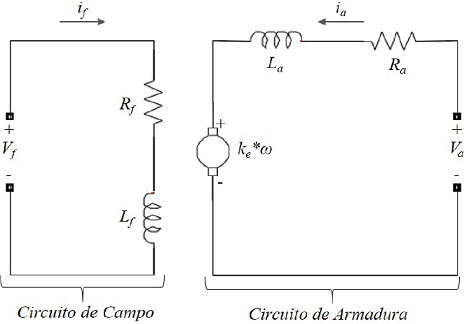
\includegraphics[width=0.5\textwidth]{img/circuito_motor_dc.jpg}
	\caption{Circuito del motor DC}
	\label{fig:circuito}
\end{figure}

Haciendo constante $i_f$ se tiene:
\[
T_m = k_m \cdot i_a(t) \qquad \text{Donde } k_m = k_1 \cdot k_f \cdot I_f
\]

Entonces:
\[
T_m(s) = k_m \cdot I_a(s)
\]

Por otro lado la cupla $T_m$ se puede escribir como:
\begin{equation}
	T_m(s) = T_L(s) + T_d(s) \rightarrow T_L(s) = T_m(s) - T_d(s) \label{T_m}
\end{equation}

Donde $T_L$ es la cupla de la carga y $T_d$ es la cupla desviadora o perturbación.  
Además:
\begin{equation}
	T_L(s) = J \cdot \theta_L(s) \cdot s^2 + B \cdot \theta_L(s) \cdot s 
	= \theta_L(s) \cdot (J s^2 + B s) \label{T_L}
\end{equation}

Además, por la ley de Faraday se genera una fuerza contraelectromotriz $V_b$ generada en los devanados de la armadura debido al movimiento del mismo dentro del campo magnético:
\[
V_b(s) = k_b \cdot \omega(s) = k_b \cdot \theta_L(s) \cdot s
\]

Por ley de tensión de Kirchhoff:
\[
V_a(s) - V_b(s) = (R_a + sL_a) \cdot I_a(s)
\]

Entonces:
\begin{equation}
	I_a(s) = \frac{V_a(s) - k_b \theta_L(s) s}{R_a + s L_a} \label{Ia}
\end{equation}

Reemplazando (\ref{T_L}) en (\ref{T_m}) haciendo $T_d = 0$ se tiene:
\begin{equation}
	\theta_L(s)(J s^2 + B s) = k_m I_a(s) \label{theta}
\end{equation}

Reemplazando (\ref{Ia}) en (\ref{theta}):
\[
\theta_L(s)(J s^2 + B s) = k_m \frac{V_a(s) - k_b \theta_L(s) s}{R_a + s L_a}
\]


Reordenando términos se llega a la función de transferencia que relaciona la posición angular de la carga en función de la tensión aplicada a la armadura:
\[
\frac{\theta_L(s)}{V_a(s)} = \frac{k_m}{s \cdot \left( L_a J s^2 + (R_a J + L_a B) s + R_a B + k_m k_b \right)}
\]

A partir de los valores obtenidos de la hoja de datos del motor y \textbf{considerando el efecto de la caja reductora ($N=40$) sobre la inercia y la fricción}, se tienen los siguientes parámetros:

\[
J_{\text{eq}} \approx \SI{1,09e-6}{\kilogram\meter\squared}
\]
\[
k_m = \SI{0,0375}{\newton\meter\per\ampere}
\]
\[
k_b = \SI{0,0374}{\volt\per\radian\per\second}
\]
\[
B_{\text{eq}} \approx \SI{2,48e-6}{\newton\meter\per\radian\per\second}
\]
\[
R_a = \SI{5,9}{\ohm}
\]
\[
L_a = \SI{250e-6}{\henry}
\]

Reemplazando estos valores en la ecuación dinámica y normalizando, obtenemos la función de transferencia del motor referida a la posición de la carga $\theta_L(s)$:

\[
\frac{\theta_L(s)}{V_a(s)} = \frac{1}{s} \cdot \frac{\num{3,44e6}}{ (s^2 + \num{2,36e4}s + \num{5,18e6})} \quad \unit{\radian\per\volt}
\]

La función de transferencia del motor que relaciona la velocidad angular en función de la tensión aplicada a la armadura derivando la ecuación anterior:

\begin{equation}
	G_{motor} = \frac{\omega_L(s)}{V_a(s)} =  \frac{\num{3,44e6}}{ (s^2 + \num{2,36e4}s + \num{5,18e6})} \quad \unit{(\radian\per\second)\per\volt} 
\end{equation}

Factorizando la ecuación se tiene:
\begin{equation}
	G_{motor} = \frac{\omega_L(s)}{V_a(s)} =  \frac{\num{3,44e6}}{ (s + 221,5)(s + 23381)} \quad \unit{(\radian\per\second)\per\volt} \label{eq:fdt_motor}
\end{equation}

\subsubsection{Modelo matemático del sensor rotativo incremental}
\label{sensor}
Un sensor rotativo (encoder) es un dispositivo que convierte el movimiento rotacional en señales eléctricas generando pulsos que indican cambios de posición, en este caso se trata de un sensor incremental, esto significa que genera un número específico de pulsos por centímetro recorrido. La función de transferencia de este sensor $H(s)$ relaciona la posición angular física de la cortina $\theta_L(s)$ en radianes con la señal digital discreta en pulsos. 

Para determinar esta relación, primero analizamos la resolución lineal del sistema. Calculamos la distancia recorrida por cada pulso del sensor ($DPP$), considerando el radio del eje ($r = \SI{0,015}{\meter}$) y la resolución del sensor ($N = 1024$ pulsos/rev):
\[
DPP = \frac{\text{circunferencia}}{\text{pulsos por rev.}} = \frac{2\pi \cdot r}{N} = \frac{2\pi \cdot 0,015 \text{ m}}{1024} \approx 9,2039 \cdot 10^{-5} \text{ m/pulso}
\]

Teniendo en cuenta la relación de transmisión de la caja reductora ($N_{red} = 40$) y la altura total de la cortina ($1,2$ m), la cantidad máxima de pulsos acumulados para el recorrido completo es:

\[
\text{Cuentas}_{\text{max}} = \frac{\text{Distancia Total} \cdot N_{red}}{DPP} = \frac{1,2 \text{ m} \cdot 40}{9,2039 \cdot 10^{-5} \text{ m/pulso}} \approx 521518 \text{ pulsos}
\]

Por otro lado, la ganancia de realimentación $H(s)$ se define como la relación entre la cantidad de pulsos generados y el desplazamiento angular de la carga. Dado que por cada revolución de la cortina ($2\pi$ radianes), el motor da 40 vueltas y el encoder genera $1024$ pulsos por vuelta:
\[
H(s) = \frac{\text{Pulsos}(s)}{\theta_L(s)} = \frac{N_{red} \cdot N_{encoder}}{2\pi} = \frac{40 \cdot 1024}{2\pi}\text{pulsos/rad}
\]

\begin{equation}
	H = H_{\text{Encoder}} \approx 6519 \text{ pulsos/rad} \label{eq:fdt_realimentacion}
\end{equation}

De esta manera, el bloque de realimentación en el diagrama entrega una señal en pulsos que es directamente comparable con el setpoint establecido por software.

\subsubsection{Modelo matemático del conversor de pulsos a voltios}

La función de esta etapa es realizar la interfaz entre el dominio digital (error en pulsos) y el dominio analógico de potencia (tensión de control en voltios), esta etapa es implementada mediante un Arduino.

Dado que el driver de potencia requiere una señal de entrada en el rango de \SI{0}{\volt} a \SI{5}{\volt}, y el comparador digital entrega un error en una magnitud de cuentas enteras (pulsos), se debe establecer una relación de equivalencia o factor de escala $K_{conv}$. Para definir esta conversión, se mapea el rango total posible de error al rango total de la señal de control. Sabemos por el análisis realizado en la sección \ref{sensor} del sensor que el recorrido total de la cortina equivale a:

\[
\text{pulsos}_{\text{max}} \approx 521518 \text{ pulsos}
\]

Y la señal de control máxima admisible antes de la saturación es:
\[
V_{\text{max}} = \SI{5}{\volt}
\]

Por lo tanto, se define la ganancia de conversión $K_{conv}$ como la relación lineal que vincula estas dos magnitudes máximas:
\[
K_{conv} = \frac{V_{\text{max}}}{\text{pulsos}_{\text{max}}} = \frac{\SI{5}{\volt}}{521.518 \text{ pulsos}}
\]
\begin{equation}
	K_{conv} \approx 9,587 \cdot 10^{-6} \quad \text{V/pulso} \label{eq:fdt_conv}
\end{equation}

\subsubsection{Modelo matemático del Driver de Potencia}

Dado que la tensión nominal del motor es de \SI{24}{\volt} y el Arduino opera con señales lógicas de \SI{5}{\volt}, se requiere una etapa de potencia para acondicionar y suministrar la energía necesaria al motor. Este dispositivo opera mediante la técnica de Modulación por Ancho de Pulso (PWM), de esta manera se logra conmutar la tensión entre 0 V y 24 V a partir del porcentaje del ciclo de trabajo del pulso.
Como la frecuencia de conmutación es muy superior a las dinámicas eléctrica y mecánica del motor, éste no sigue las variaciones instantáneas, sino el valor promedio de la tensión aplicada. Por lo tanto se puede modelar de la siguiente forma:

\[
V_{\text{out}}(t) = D(t) \cdot V_{dc} \rightarrow V_{\text{out}}(t) = \frac{V_{\text{in}}(t)}{\SI{5}{\volt}} \cdot \SI{24}{\volt}
\]

\[
K_{\text{driver}} = \frac{V_{\text{out}}}{V_{\text{in}}}= \frac{\SI{24}{\volt}}{\SI{5}{\volt}} = 4,8
\]

\subsubsection{Diagrama de bloques}
A continuación se muestra el diagrama de bloques del sistema

\begin{figure}[h]
	\centering
	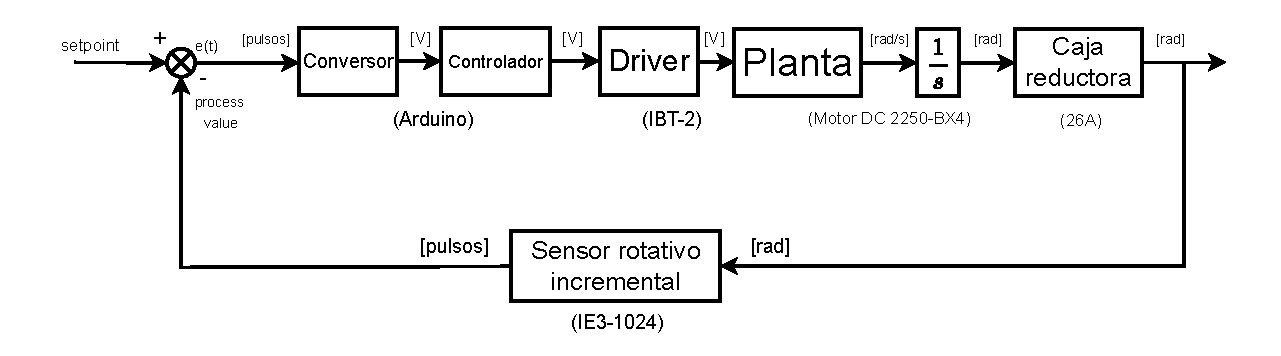
\includegraphics[width=1\textwidth]{img/diagrama_de_bloques_lazo_cerrado.pdf}
	\caption{Diagrama de bloques del sistema}
	\label{fig:diagrama de bloques del sistema}
\end{figure}


Del diagrama de bloques se deduce la función de transferencia de la trayectoria directa:

\begin{equation}
	G(s) = K_{\text{conv}} \cdot K_{\text{driver}} \cdot G_{\text{motor}} \cdot \frac{1}{s} = \frac{\num{3,44e6}}{s \cdot (s^2 + \num{2,36e4}s + \num{5,18e6})} \quad \unit{\radian\per\volt}
\end{equation}

y luego la función de transferencia a lazo abierto del sistema:

\begin{equation}
	FT_{LA} = G(s)\cdot H = \frac{\num{1,028e6}}{s\cdot(s^2+\num{2,36e4}\cdot s + \num{5,18e6})}\quad \unit{\radian\per\volt} \label{eq:fdla}
\end{equation}

\subsubsection{Análisis de estabilidad absoluta}
\label{analisis_est}
La estabilidad absoluta de la planta se determina analizando la ubicación de los polos de la función de transferencia a lazo abierto $FT_{LA}$ en el plano complejo $s$. 

De la ecuación \ref{eq:fdla}, se obtiene el polinomio denominador:

$$D(s) = s \cdot (s^2 + 2,36\cdot10^4 s + 5,18\cdot10^6)$$

Las raíces de este polinomio son:

\[
s_1 = \num{0}, \qquad
s_2 = \num{-221,5}, \qquad
s_3 = \num{-23381}
\]

Dado que todos los polos poseen parte real negativa o nula, y existe un polo simple estrictamente en el origen ($s_1 = 0$), se concluye que la planta es \textbf{marginalmente estable.}

Físicamente, esto significa que el sistema se comporta como un integrador puro: ante una entrada acotada de tensión constante (escalón), la velocidad angular se estabilizará, pero la posición angular crecerá indefinidamente (rampa) sin llegar nunca a un valor estacionario por sí sola. \textbf{Esto evidencia la necesidad de implementar un lazo de control realimentado} para gobernar la posición de la cortina.


\subsubsection{Análisis de la respuesta temporal de la planta}
Con el objetivo de verificar los parámetros dinámicos del modelo matemático obtenido, se simuló la respuesta temporal de la planta ante una entrada escalón de tensión de $\SI{5}{V}$ ($\SI{24}{V}$ en el motor) operando a lazo abierto como se muestra en el siguiente diagrama de bloques y se observó la respuesta temporal de la velocidad angular

\begin{figure}[h]
	\centering
	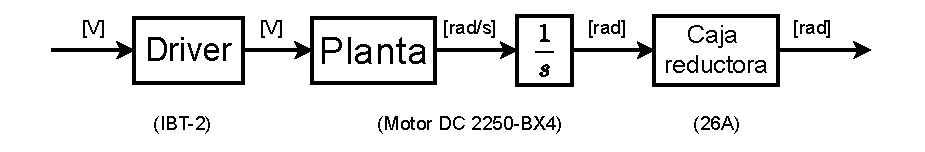
\includegraphics[width=1\textwidth]{img/diagrama_de_bloques_planta.pdf}
	\caption{Diagrama de bloques de la planta a lazo abierto}
	\label{fig:diagrama de bloques de la planta}
\end{figure}

\begin{figure}[h]
	\centering
	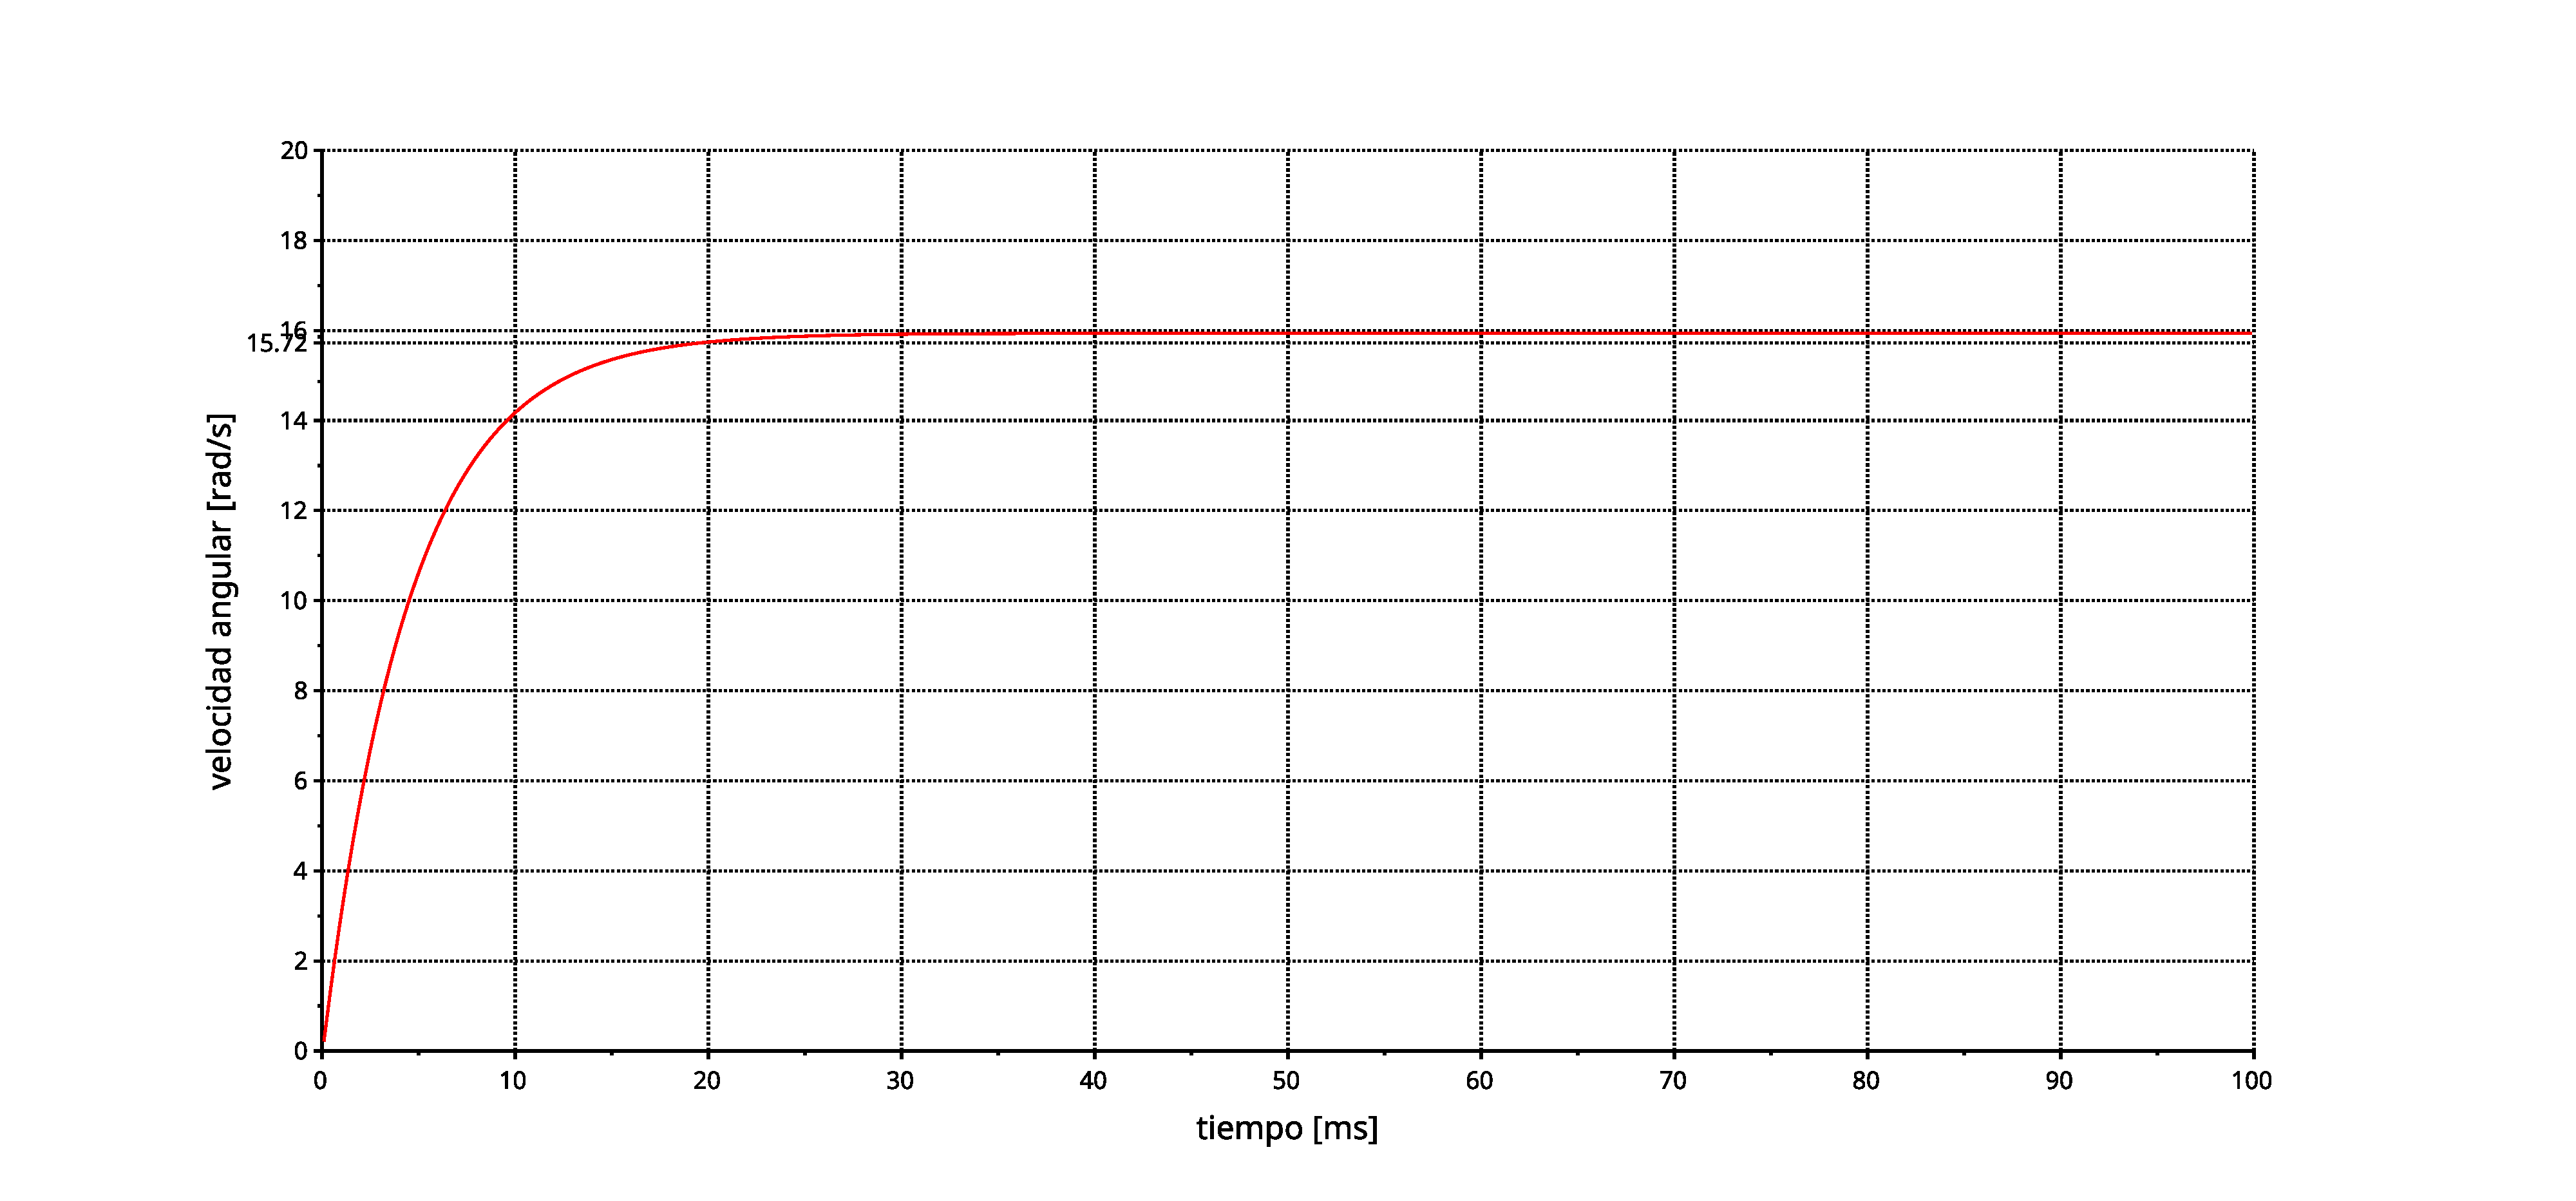
\includegraphics[width=1\textwidth]{img/respuesta_escalon_24V.pdf}
	\caption{Respuesta temporal de la planta ante un escalón de 24V}
	\label{respuestatemporalplanta}
\end{figure}

Como se puede observar en la Figura \ref{respuestatemporalplanta}, la velocidad angular alcanza el valor de $\SI{15,72}{\radian\per\second}$ (ingresando a la banda del $\SI{2}{\percent}$ de tolerancia del valor final de aproximadamente $\SI{16,02}{\radian\per\second}$) en un tiempo de establecimiento de aproximadamente 20 milisegundos.

En la sección \ref{pdominantes} se calcula el valor teórico de la constante de tiempo mecánica ($\tau_m \approx 4,5$ ms), considerando el criterio de 4 constantes de tiempo para el cual se llega al $\SI{98,3}{\percent}$ del valor final:

\[
t_s = 4 \cdot \tau_m = 4 \cdot \SI{4,5}{\milli\second} = \SI{18}{\milli\second}
\]

Coincide de manera aproximada con el valor obtenido en la simulación de respuesta transitoria.

El valor final coincide con el teórico, el cual se obtiene a partir de la velocidad angular máxima calculada en la ecuación \ref{eq:va_max} dividida por el valor de la relación de transmisión de la caja reductora:

\[
\omega_f =  \frac{\omega_{\text{max}}}{N} = \frac{\SI{641,7}{\radian\per\second}}{40} = \SI{16,04}{\radian\per\second}
\]

De esta manera \textbf{se verifica el modelo matemático de la planta a partir de la respuesta temporal}

\subsubsection{Polos dominantes}
\label{pdominantes}
Los polos dominantes de un sistema son aquellos polos de la función de transferencia a lazo abierto que se encuentran más cercanos al eje imaginario del plano complejo y son los que tienen mayor impacto en la respuesta temporal del sistema.
A partir de la función de transferencia de lazo abierto $FT_{LA}$ (ecuación \ref{eq:fdla}), se identifican las raíces del denominador (polos) que gobiernan la dinámica natural del sistema:

\[
s_1 = \num{0}, \qquad
s_2 = \num{-221,5}, \qquad
s_3 = \num{-23381}
\]

Por lo tanto \textbf{el polo dominante se encuentra en $s_2 = \num{-221,5}$} correspondiente a la dinámica mecánica del motor, a partir de éste se determina la constante de tiempo mecánica:
\[
	\tau_m = \frac{1}{-s_2} = \frac{1}{221,5} \approx \SI{4,5}{\milli\second} 
\]

\subsubsection{Error en estado estable}
\label{ees}


El error en estado estable se define como el valor al que tiende la señal de error $e(t)$ cuando el tiempo tiende a infinito. En un diagrama de bloques estándar, esta señal representa la diferencia entre la entrada de referencia (\textit{setpoint}) $R(s)$ y la señal de realimentación (\textit{process value}).

\[
e_{ss} = \lim_{t \to \infty} e(t) = \lim_{s \to 0} s \cdot E(s) = \lim_{s \to 0} \frac{s \cdot R(s)}{1 + G(s)H(s)}
\]

El tipo de sistema determina el error en estado estable en relación con el tipo de entrada de referencia. En nuestro caso como se puede observar en la función de transferencia a lazo abierto (ecuación \ref{eq:fdla}), tenemos un polo en $s=0$, esto significa que el sistema es de tipo $1$, \textbf{por lo tanto el error en estado estable para una entrada tipo escalón es nulo y para una entrada tipo rampa el error es constante}
